
\title{Separation and imaging of seismic diffractions using a localized rank-reduction method with adaptively selected ranks}

\renewcommand{\thefootnote}{\fnsymbol{footnote}}

\author{Hang Wang \footnotemark[1], Xingye Liu \footnotemark[2] and Yangkang Chen\footnotemark[1]}

\ms{GEO-2020} %\ms{GJI-2019}

\address{
\footnotemark[1]
Key Laboratory of Geoscience Big Data and Deep Resource of Zhejiang Province\\
School of Earth Sciences\\
Zhejiang University\\
Hangzhou, Zhejiang Province, China, 310027\\
chenyk2016@gmail.com \& 18328504171@163.com\\
\footnotemark[2]
College of Geology and Environment\\
Xi’an University of Science and Technology\\
Xi’an, Shaanxi Province, China, 710054 \\
lwxwyh506673@126.com\\
Corresponding Author: Yangkang Chen (chenyk2016@gmail.com) 
}

\lefthead{Wang et al.}
\righthead{Separation and imaging of seismic diffractions}

\DeclareRobustCommand{\dlo}[1]{}
\DeclareRobustCommand{\wen}[1]{#1}

\begin{abstract}
Seismic diffractions are some weak seismic events hidden within the more dominant reflection events in a seismic profile. Separating diffraction energy from the post-stack seismic profiles can help infer the subsurface discontinuities that generate the diffraction events. The separated seismic diffractions can be migrated with a traditional seismic imaging method or a specifically designed migration method to highlight the diffractors, i.e., the diffraction image. Traditional diffraction separation methods based on the the underlying plane-wave assumption are limited by either the inaccurate slope estimation or the plane-wave assumption of the PWD filter, and thus will cause reflection leakage into the separated diffraction profile. The leaked reflection energy will deteriorate the resolution of the subsequent diffraction imaging result. Here, we propose a new diffraction separation method based on a localized rank-reduction method. The localized rank-reduction method assumes the reflection events to be locally low-rank and the diffraction energy can be separated by a rank-reduction operation. Compared with the global rank-reduction method, the localized rank-reduction method is more constrained in selecting the rank and is free of separation artifacts. We use a carefully designed synthetic example to demonstrate that the localized rank-reduction method can help separate the diffraction energy from a post-stack seismic profile with both kinematically and dynamically accurate performance. 
\end{abstract}

\maketitle


%\section{Keywords}
%key1,key2,key3

\section{Introduction}
Diffraction is a very common \dlo{type of seismic waves which}\wen{wave type that} can be observed in almost every \wen{seismic} data set. \dlo{The small-scale}\wen{Small-scale} geological bodies (such as \dlo{salt dome,} faults and fractures in carbonate rocks\dlo{, etc.}) are the main \dlo{reasons for the appearance of it}\wen{cause}. As the simple hydrocarbon reservoirs have been fully explored and exploited, the unconventional hydrocarbon reservoirs controlled by these small geological bodies \dlo{gradually draw}\wen{are now drawing} attentions of\dlo{ the} exploration geophysicists. The well-preserved diffraction can provide rich information about these reservoirs \cite[]{Gelius1995limit,Landa1998moni,decker2017diffraction}. However, in the traditional seismic exploration workflow, \dlo{the }diffractions \dlo{is}\wen{are} treated as a kind of noise and removed from the original data. \dlo{Additionally, because the amplitude of diffraction is usually weaker than that of reflection wave, it will create more difficulties in the final imaging of it.}\wen{In addition, the weakness of diffraction amplitudes leads to final imaging challenges.} Thus, \dlo{the}\wen{developing} effective and accurate methods for diffraction imaging \dlo{are badly needed by the oil industry in the future}\wen{would be a beneficial goal}. 

Generally, the key of diffraction imaging is to \wen{accurately} separate the reflection and diffraction\dlo{ accurately}. Based on this idea, many separating methods have been proposed \dlo{in the past few years. These approaches, according to their mathematical algorithms, can be roughly divided into two}\wen{, which can be divided into two main categories according to their mathematical algorithms,} path-summation-based methods and \dlo{the other is the} wave-equation-based methods.  Additionally, some other approaches such as machine learning \cite[]{Tschannen2020dp} are also effective tools for imaging the diffraction \cite[]{Protasov2019spectral}.

For the path-summation-based methods, the traveltime (event shape) is of great importance to the separation of reflection and diffraction \cite[]{Kanasewich1988dis,Santos2012Tomo}. \cite{Berkovitch2009multi} \dlo{used}\wen{use} a multifocusing algorithm to separate \dlo{the diffraction and reflection}\wen{diffractions from reflections by designing}\dlo{. They designed} a novel time-correction formula\dlo{, which contains angle and radius parameters,} to approximate the diffraction events. This method can make the energy of diffraction more focused while scattering that of reflection in the stacking result. \cite{Dell2011crs} separate diffraction and reflection \wen{energy} in the time domain using a common-reflection-surface algorithm. Different synthetic examples showed the validity of this method. \cite{Waheed2013ti} propose a new method for fitting the \dlo{traveltime of the diffraction}\wen{diffraction traveltimes} in the TI media. This approach can accelerate the traditional process for solving equation and lower the computational complexity. Additionally, it adaptively selects the best parameters for the traveltime equation without complex modeling processes. \cite{Asgedom2013co} combine two novel algorithms, i.e., the modified common‐reflection‐surface method and the replacement‐media technique, to enhance the weak diffraction in the strong reflection background. \dlo{The stability of this method under different data qualities was also tested. }\cite{Coimbra2018fo} propose  \dlo{anew equation to describe the traveltime of diffraction called }\wen{the} finite-offset double-square-root diffraction traveltime equation\dlo{. Via this precise fitting result,}\wen{that can accurately separate} diffraction\dlo{ can be separated properly} from the background reflection. A simplified version was also proposed to accelerate the calculation of the equation parameters while keeping the quality of result unchanged. The synthetic and field data \wen{results} \dlo{showed}\wen{show} the outstanding performance of this improvement. \cite{bakhtiari2018common} compare the influence of pre-stack and post-stack diffraction separation to imaging performance, and showed that the \dlo{pre-stack}\wen{former} method based on the wavefront attributes can help improve the illumination compared with the \dlo{post-stack}\wen{latter} method.  \cite{Zhengwei2019vtd} design a vertical traveltime difference gather and its plus version. Compared with the traditional two-dimensional dip gather, this gather has the advantage of occupying less storage space. After Kirchhoff time migration, the diffraction is flattened, and the reflection events still have \dlo{the upward dip}\wen{upward dip}. By this difference, the reflection can be cut off, which will further strengthen \dlo{the amplitude of diffraction}\wen{recovered diffraction amplitudes}. \dlo{Finally, the result of diffraction imaging will be generated. }\cite{merzlikin2019least} introduce the separation of diffraction into an inversion framework, and designed a new decomposition algorithm by combining Kirchhoff modeling, plane-wave deconstruction and an integral operator. This method \wen{simultaneously} separates weak diffraction and strong reflection accurately, \dlo{and suppresses the noise sufficiently at the same time}\wen{while sufficiently supressing noise}. \cite{Benjamin2019cohe} design an adaptive filter to separate diffraction in the background of strong reflection. This method is mainly based on the summation of reflection data rather than diffraction data, and uses a variety of wavefront filters in the stacking domain to separate diffraction and reflection. \dlo{Through the examples of seismic data and GPR, they demonstrated}\wen{Using seismic and GPR data examples, they demonstrate} that this method could recover weak diffraction signals effectively. 

\dlo{For the wave-equation-based}\wen{Wave-equation-based} methods\dlo{, they} take all the wavefield information into consideration \cite[]{Sava2005wave,Hemin2019gpr}. \cite{Klokov2012dip} \dlo{gave}\wen{derive} a novel analytical equation to accurately separate the diffraction and reflection. After the migration process, the Radon transform can distinguish the diffraction effectively by its shape feature. This method is very stable on both synthetic and field data examples. \cite{Zhang2014opening} image the weak diffraction in the shot and opening-angle gathers by muting the strong reflection and enhancing the weak diffraction. This method \dlo{keeps obtaining the}\wen{generates} satisfactory results even if the diffraction interferes with the reflection. The velocities for migration can be gradually updated based on the migrated results to achieve the best result. The real and synthetic data all showed the validity of this method. \cite{Liu2016wave} propose a fast migration method for the imaging of diffraction. They first use linear Radon transform to obtain the local plane waves\dlo{. Then, implemented}\wen{, and then implement} the zero-lag correlation between these plane waves and incident waves. The final diffraction image \dlo{was}\wen{is} generated after the energy of reflected wave was attenuated by a median filter. \cite{Dongliang2019wave} divide the wavefield into two parts, left and right, by using reverse time migration. Based on the fact that the reflection is always related to a specific dip angle, and can only exist in either the left or right wave field. However, due to the nature of diffraction, \dlo{it can}\wen{associated energy will simultaneously} appear in \dlo{two}\wen{both} components at \dlo{the same time. By the} point-by-point multiplication between two components\dlo{, the}\wen{ can suppress} reflection \dlo{can be suppressed }while the imaging result of diffraction\dlo{ will be highlighted}.

\cite{fomel2007} proposes a two-step diffraction separation and imaging framework. \dlo{In the first step, the}\wen{The first step separates} diffraction and reflection wavefields \dlo{are separated }based on the spatial coherence using the plane-wave destruction (PWD) method. The PWD method assumes that the reflection waves have better spatial coherence than the diffraction waves, and thus can be predicted by neighbor traces following the smooth local slope field. In the second step, the separated diffraction waves are migrated using different velocities. Their corresponding focusing performance on the images are measured to determine the \dlo{best }migration velocity \dlo{that results in the best focused image.}\wen{that optimally focuses the image.} In this way, one can achieve simultaneous velocity estimation and diffraction imaging. Based on this framework, the \dlo{separation of diffraction  waves}\wen{diffraction separation} becomes a pure signal processing task, where no prior subsurface velocity models are required. Thus, this method is easy to apply and sometimes can obtain very good performance in real data applications. \wen{In a similar framework, \cite{zhou2017enhancing} and \cite{zhou2018seismic} develop a method to extract diffractions from high-resolution coal seismic data using localized moving-average-error filter (MAEF) to flattened reflection seismic data and or along the reflection dips based on the estimated dip by gradient calculation.} However, the success of this method depends on  the accuracy of the estimated slope. Because of the smoothness of the local slope, \dlo{the reflection waves in complicated areas or with small dip angles can also be separated by the PWD method, which further results in a poor resolution of the migrated diffraction image}\wen{there is leakage of reflection energy into the diffraction estimate which contaminates the imaging results}.  

In this paper, we propose a new diffraction separation method based on a localized rank-reduction method (LRR). The LRR method \dlo{is also based on the assumption of local plane waves}\wen{also uses a local plane-wave assumption}, but \dlo{can bypass}\wen{bypasses} the step of slope estimation. The compromise between the removal of diffractions and preservation of reflections is controlled by the rank in each local window. We propose an adaptive rank-selection method for each localized window to select the \dlo{best}\wen{optimal} cut-off rank that best distinguishes between reflections and diffractions. After the diffraction separation step, an migration operation is applied to obtain the migration diffraction image, e.g., by Kirchhoff migration \cite[]{fomel2002antialiasing}, velocity continuation \cite[]{fomel20037}\dlo{, etc}. 

The paper is organized as follows: we first introduce the principles of the LRR method. Then, we introduce how we adaptively select the ranks in each local window. The hybrid LRR and adaptive rank selection method is referred to as the localized rank-reduction method with adaptively chosen ranks (LRRA). Next, we use several representative examples to demonstrate the performance of the proposed diffraction separation method, and more importantly how the new method can improve the resolution and fidelity of the final image. \dlo{We finally draw some key conclusions at the end.  }

\section{Methods for adaptively separating diffractions}
The ranks or the singular (characteristic) values of the matrix data are calculated by the SVD method and are measures of the different dipping events within the matrix data (seismic data). This approach is well-known as the matrix pencil method (MPM) \cite[]{jain1974filter,hua1991svd,sarkar1995using}. The MPM approach has been used for dispersion estimation of sonic logging data \cite[]{lang1987estimating,ekstrom1996dispersion}\dlo{. It is assumed}\wen{, and assumes} that the first a few characteristic values are associated with the reflection data while the rest are related to diffractions. Therefore, we can estimate or separate reflections and diffractions from recorded seismic data by matrix rank reduction or truncation. As the seismic events are not necessarily linear or follow plane wave assumption, we propose to apply the matrix rank reduction approach on windowed data to better approximate the \wen{plane-wave} assumption for the reflection data. We call this method a localized rank-reduction method.
\subsection{Localized rank-reduction method}
%For a given regular grid, the relationship between the complete earthquake data $\mathbf{d}\in\mathbb{R}^{N_tN_xN_y\times1}$
%
%$\mathbf{R}$ represents the reconstruction filter and is usually applied in the frequency-space domain in the rank-reduction methods \cite[]{Vicente2011Simultaneous}.
Without the loss of generalization, we introduce the theory of the rank-reduction method in the case of a 3D problem. The 2D problem is just special case of the 3D problem \dlo{when the number of crossline traces is 1}\wen{with a single crossline trace}. In the rank-reduction method, a pre-transformed matrix, e.g., the block Hankel matrix, is assumed to be of low rank. Then the goal becomes to extract the principal components of the pre-transformed matrix, i.e., the reflection signals, and separate the diffractions that usually corresponds to the inessential components due to \dlo{the less}\wen{lower} spatial coherence.

Assuming that the tensor form of the input 3D seismic data is $D(x,y,t)$, the corresponding form in frequency-space domain \dlo{be}\wen{is} obtained after Fourier transform and can be expressed as $D(x,y,f)$.  For each frequency slice, we map the frequency domain data into several block Hankel matrices. This process is referred as Hankelization \cite[]{mssa,weilin2016dmssa,amir2017grsl}. Given a frequency $f$, the Hankel matrix can be constructed as 
\wen{\begin{align} \label{eq:Rif} 
\mathbf{H}_i(f)=
\begin{bmatrix}
D(i,1,f)&D(i,2,f)&\cdots&D(i,Q_y,f)\\
D(i,2,f)&D(i,3,f)&\cdots&D(i,Q_y+1,f)\\
\vdots&\vdots&\ddots&\vdots\\
D(i,P_y,f)&D(i,P_y+1,f)&\cdots&D(i,N_y,f)
\end{bmatrix},
\end{align}
where the subscript $i$ is the row and $\mathbf{H}_i(f)$ is the Hankel matrix in frequency domain corresponding to the data matrix in frequency-space domain $D(x,y,f)$.
$P_y=\lfloor N_y/2\rfloor+1$, $Q_y=N_y-P_y+1$ and $\lfloor \cdot \rfloor$ \dlo{is reserving integer part operator}\wen{denotes the integer part of an input argument}. $N_y$ denotes the number of traces in the $y$ direction. }

\wen{Then, the corresponding block Hankel matrix can be inserted with equation \ref{eq:Rif}
\begin{align} \label{eq:H} 
\mathbf{B}(f)=
\begin{bmatrix}
\mathbf{H}_1(f)&\mathbf{H}_2(f)&\cdots&\mathbf{H}_{Q_x}(f)\\
\mathbf{H}_2(f)&\mathbf{H}_3(f)&\cdots&\mathbf{H}_{Q_x+1}(f)\\
\vdots&\vdots&\ddots&\vdots\\
\mathbf{H}_{P_x}(f)&\mathbf{H}_{P_x+1}(f)&\cdots&\mathbf{H}_{N_x}(f)
\end{bmatrix},
\end{align}
where $P_x=\lfloor N_x/2\rfloor+1$, $Q_x=N_x-P_x+1$.  $N_x$ denotes the number of traces in the $x$ direction.}

The rank-reduction can be achieved by minimizing the following objective function
\begin{align} \label{eq:obj} 
\begin{split}
\text{min} \quad &O=\|\mathbf{B}(f)-\mathbf{L}(f)\|^2_F\\
\text{subject to} \quad&\text{rank}(\mathbf{L}(f))=L,
\end{split}
\end{align} 
where $\mathbf{L}(f)$ denotes the low-rank section corresponding to $\mathbf{B}(f)$. $L$ denotes the optimal rank parameter. The above objective function can be conveniently minimized by the well-known singular value decomposition (SVD). Therefore, the SVD of block Hankel matrix $\mathbf{B}(f)$ can be expressed as
\begin{equation} \label{eq:svd}
\mathbf{B}(f)=\mathbf{U}\mathbf{\Sigma}\mathbf{V}^T,
\end{equation}
where $\mathbf{U}=[\mathbf{u}_1,\mathbf{u}_2,\cdots,\mathbf{u}_N]$ is a left singular matrix, $\mathbf{\Sigma}=[{\sigma}_1,{\sigma}_2,\cdots,{\sigma}_N]$ is a singular matrix and $\mathbf{V}=[\mathbf{v}_1,\mathbf{v}_2,\cdots,\mathbf{v}_N]$ is a right singular matrix. $\sigma_i$ represents the $i$th singular value, and $N$ represents the number of columns of $\mathbf{B}(f)$. Next, the rank-reduced matrix $\mathbf{L}(f)$ can be calculated by extracting the first $L$ principal components, i.e.,
\begin{equation}\label{eq:solution}
\mathbf{L}(f)=\sum^L \limits_{i=1} {\sigma}_i\mathbf{u}_i\mathbf{v}_i^T.
\end{equation}

Then, the solved low-rank Hankel matrix is rearranged to a vector form according to inverse Hankelization process. The rank-reduction method can be summarized as follows:
\begin{equation}
\label{eq:rr}
\begin{split}
\mathbf{R} &=\mathcal{F}^{-1}\mathbf{T}\mathcal{F}\mathbf{D},\\
\mathbf{T} &=\mathcal{A}\mathcal{L}\mathcal{H},
\end{split}
\end{equation}
where $\mathbf{R}$ denotes the separated reflections. The separated diffractions can directly obtained by $\mathbf{D}-\mathbf{R}$. $\mathcal{F}$ and $\mathcal{F}^{-1}$ denote forward and inverse Fourier transforms. 

In equation \ref{eq:rr}, filter $\mathbf{T}$ is referred to as the frequency-domain rank-reduction operator, containing the Hankelization $\mathcal{H}$, principal component extraction $\mathcal{L}$ and inverse Hankelization process $\mathcal{A}$.   Because of the complexity of seismic data, the plane-wave assumption is only valid locally. Thus, it is more appropriate to apply the rank-reduction method locally, i.e., in local windows:
\begin{equation}
\label{eq:lrr}
\mathbf{R} =\mathcal{W}^{-1}\mathcal{F}^{-1}\mathbf{T}\mathcal{F}\mathcal{W}\mathbf{D},
\end{equation}
where $\mathcal{W}$ and $\mathcal{W}^{-1}$ denote a pair of windowing and reconstruction operators. 

\subsection{Automatic rank selection}
In order to obtain a satisfactory result, an appropriate $L$, referred to the rank, should be cautiously selected.  A big value of $L$ will lead to preserving all components, while a small value of the rank will cause damage on the preserved reflections by the rank-reduction filter.  In the first case, negligible diffraction energy \dlo{could be}\wen{are} separated. In the second case, only the most coherent wave components, e.g., horizontal waves, \dlo{can be}\wen{are} preserved \cite[]{yangkang2017lsrtm,yangkang2019nc}. Thus, there will be a strong mixture between the separated reflections and diffractions. Therefore, the determination of rank parameter is difficult and traditional methods \dlo{such as the approaches based on the events that have distinct slowness}\wen{that exploit distinct event slowness} \cite[]{Vicente2011Simultaneous} cannot perform well in complicated situations. 

For the rank-reduction filtering, an alternative method is to adaptively and automatically select the rank parameter based on the features and complexity of the data. In the singular spectrum, the singular values of signals and noise are discrepant. The cut-off rank in singular value spectrum can indicate the separation of signal and noise energy. On this basis, we use an adaptive strategy to optimize the rank \cite[]{yangkang2017lsrtm,yangkang2019nc}.  At first, we define a singular value ratio (SVR):
\begin{equation} 
\label{eq:svr}
m_i=\dfrac{\sigma_i}{\sigma_{i+1}},i=1,2,\cdots,N-1,
\end{equation}
where $\{m_i\}$ denotes the SVR sequence, and $N$ is the length of the singular spectrum. Then, the rank $L$ can be calculated by maximizing the  SVR sequence, i.e.,
\begin{equation} \label{eq:svr}
\hat{L}=\text{arg} \max\limits_i\quad m_i.
\end{equation}

A detailed analysis of the LRRA method on the diffraction separation problem is presented in the next section. In addition, we will aslo comprehensively analyze the reliability of the adaptive rank selection strategy in accurately separating diffractions from reflection waves in the next section. 


\inputdir{synth}
\multiplot{3}{s-datai,s-diffr,s-data}{width=0.45\textwidth}{(a) Simulated reflection data. (b) Simulated diffraction data. (c) Simulated zero-offset data containing both reflections and diffractions.}


\multiplot{4}{s-pwd-s,s-pwd-n,s-lrra-s,s-lrra-n}{width=0.45\textwidth}{(a) Separated reflections using PWD method. (b) Separated diffractions using PWD method. (c) Separated reflections using LRRA method.  (d) Separated diffractions using LRRA method. }

\plot{s-dip0}{width=0.6\textwidth}{Estimated local slope from the zero-offset data shown in Figure \ref{fig:s-data}, which is used for \dlo{the plane-wave destruction}\wen{PWD analysis}. Note that both reflection and diffraction slopes are revealed in this map.}

\multiplot{4}{s-lrr-N2-s,s-lrr-N3-s,s-lrr-N4-s,s-lrr-N5-s}{width=0.45\textwidth}{Separated reflections using LRR method with (a) N=2, (b) N=3, (c) N=4, (d) N=5. }

\multiplot{4}{s-lrr-N2-n,s-lrr-N3-n,s-lrr-N4-n,s-lrr-N5-n}{width=0.45\textwidth}{Separated diffractions using LRR method with (a) N=2, (b) N=3, (c) N=4, (d) N=5. }

\multiplot{4}{s-grr-N5-s,s-grr-N10-s,s-grr-N16-s,s-grr-N25-s}{width=0.45\textwidth}{Separated reflections using GRR method with (a) N=5, (b) N=10, (c) N=16, (d) N=25. }

\multiplot{4}{s-grr-N5-n,s-grr-N10-n,s-grr-N16-n,s-grr-N25-n}{width=0.45\textwidth}{Separated diffractions using GRR method with (a) N=5, (b) N=10, (c) N=16, (d) N=25. }

\multiplot{4}{s-mig-true,s-mig0,s-mig-tra,s-mig}{width=0.45\textwidth}{True diffraction image (a) and migration results of (b) traditional method, (c) PWD method, and (d) LRRA method.}


\section{Comparison of Diffraction Imaging}
\subsection{Synthetic test}
In order to test the effective performance of the proposed localized rank-reduction method\dlo{. We}\wen{, we} use a synthetic and two real data examples to show the better diffraction separation performance of the LRRA method, and compare it with the state-of-the-art PWD based method. To demonstrate the advantages of the localized-processing and automatic rank selection strategies, we compare the rank-reduction methods in different cases, considering local or global processing, and fixed or adaptive rank selection.

\dlo{The first example is a synthetic test, as presented in Figure \ref{fig:s-datai,s-diffr,s-data}.} We first generate the reflection data from five reflection surfaces by \dlo{the }Kirchhoff modeling \dlo{, and plot it in Figure \ref{fig:s-datai}}\wen{(Figure \ref{fig:s-datai})}. Then, we generate the diffraction data from a set of diffraction points \dlo{, and plot it in Figure \ref{fig:s-diffr}}\wen{(Figure \ref{fig:s-diffr})}. We sum the reflection and diffraction data to output the simulated zero-offset data \dlo{, as shown in Figure \ref{fig:s-data}}\wen{(Figure \ref{fig:s-data})}. The size of the zero-offset dataset is 800$\times$501. The temporal sampling is 4 ms and \dlo{space}\wen{spatial} sampling is 0.02 km. Note that the same synthetic data \dlo{was}\wen{were} also used in \cite{merzlikin2019least}. We show the results from the PWD method \cite[]{fomel2007} and the proposed LRRA method in Figure \ref{fig:s-pwd-s,s-pwd-n,s-lrra-s,s-lrra-n}. \dlo{The left column of Figure \ref{fig:s-pwd-s,s-pwd-n,s-lrra-s,s-lrra-n} compares}\wen{Figures \ref{fig:s-pwd-s} and \ref{fig:s-lrra-s} compare} the separated reflections\dlo{ and the right column compares}\wen{while Figures \ref{fig:s-pwd-n} and \ref{fig:s-lrra-n} show} the separated diffractions. It is clear that the PWD method \dlo{(top row)}\wen{(Figures \ref{fig:s-pwd-s} and \ref{fig:s-pwd-n})} causes significantly more residual diffractions in the separated reflections than the proposed LRRA method \dlo{(bottom row)}\wen{(Figures \ref{fig:s-lrra-s} and \ref{fig:s-lrra-n})}. Correspondingly, the separated diffractions of the PWD method are much weaker than those from the proposed LRRA method. We attribute the unsatisfactory performance of the PWD method to the failure in distinguishing between the reflections and diffractions in the local slope map, as plotted in Figure \ref{fig:s-dip0}. Because the slope estimation method calculates the slope for both reflections and diffractions, it is difficult to separate them for PWD diffraction separation method that relies on the slope difference. In this test, we use a local window with 200 samples in time and 100 samples in space. The window size is chosen so as to \dlo{maximize}\wen{optimize} the \dlo{separation ability}\wen{separability of}\dlo{ between} diffractions\dlo{ and}\wen{from} reflections. Based on this criterion, we choose the optimal window size based on a try-and-error strategy in practice. We move the window by half of the window size in each directions, meaning that the overlap between two neighbor windows are 50\%. We take the automatic rank selection strategy as introduced previously so we do not need to specify the rank parameter in the LRRA method. The PWD algorithm \cite{fomel2002pwd} \dlo{used }in this paper is a local algorithm, but does not use local windows. \cite{fomel2002pwd} \dlo{avoided}\wen{avoids} the use of local window strategy by designing a non-stationary dip estimation method, where the window size is substituted by the smoothing radius. \dlo{So}\wen{Thus} the only parameter that affects the slope estimation is the smoothing radius (along time and space). A larger smoothing radius corresponds to a larger local window size, i.e., smoother, and vice versa. But the smoothing radius \dlo{can}\wen{does} not result in the same effect as the local window strategy. For example, when we increase the smoothing radius to a large level, the diffraction slope shown in Figure \ref{fig:s-dip0} will be weakened. But, at the same time, the accuracy of the reflection slope will \dlo{be deteriorated}\wen{deteriorate}, thereby making the reflection not fully separated. In the opposite way, if the smoothing radius is smaller, like in this paper, the diffraction slope shows up, then the diffraction is not easy to be separated. So, this is the contradiction in tuning the PWD algorithm. In this paper, we use a smoothing radius of \dlo{10}\wen{ten} samples along both horizontal and vertical directions.


To compare the performance of the automatic rank selection strategy and manual rank selection strategy, we perform several try-and-error tests by specifying different ranks based on the LRR method. Figure \ref{fig:s-lrr-N2-s}-\ref{fig:s-lrr-N5-s} shows four separated reflection sections based on the LRR method with a fixed rank of \dlo{$N=2$ (a), $N=3$ (b), $N=4$ (c), and $N=5$ (d)}\wen{$N=[2,3,4,5]$, respectively}. Correspondingly, Figure \ref{fig:s-lrr-N2-n}-\ref{fig:s-lrr-N5-n} shows four separated diffraction sections based on the LRR method with \dlo{a fixed rank of $N=2$ (a), $N=3$ (b), $N=4$ (c), and $N=5$ (d)}\wen{the same fixed rank as Figure \ref{fig:s-lrr-N2-s,s-lrr-N3-s,s-lrr-N4-s,s-lrr-N5-s}}. From Figures \ref{fig:s-lrr-N2-s,s-lrr-N3-s,s-lrr-N4-s,s-lrr-N5-s} and \ref{fig:s-lrr-N2-n,s-lrr-N3-n,s-lrr-N4-n,s-lrr-N5-n}, we can find that the residual diffraction energy in the separated reflection sections gradually increases, and the reflection energy in the separated diffraction sections decreases, as the fixed rank increases from $N=2$ to $N=5$. All these results from the LRR method with fixed ranks \dlo{seem to be worse}\wen{appear worse} than the result from the LRRA method. For example, when $N=2$, the separated reflection section (Figure \ref{fig:s-lrr-N2-s}) is clean and free of diffraction, but the separated diffraction contains very strong reflection energy, which will significantly deteriorate the resolution of migrated diffractors in the diffraction image. When $N=5$ (Figure \ref{fig:s-lrr-N5-s}), the separated diffraction section contains pure diffraction energy, but \dlo{its}\wen{the associated} reflection section contains significant diffraction energy, thus the resulted diffraction image will not be accurate. When $N=3$ and $N=4$, it seems that the LRR method obtains a better compromise, but is less \dlo{competent}\wen{powerful in removing the diffractions} \dlo{as}\wen{than} the LRRA method\dlo{ is better separating the two components}. The worse performance of the LRR method with a fixed rank compared with the LRRA method with automatically selected ranks is due to the rank inconsistency problem \cite[]{shaohuan2017gji}, i.e., the optimal ranks in each localized processing window are different and thus a globally defined rank cannot suit each localized window. In addition to the superior perfomance, LRRA method also avoids the try-and-error process for rank selection and is more convenient to apply. 

We also compare the performance of diffraction separation based on a global rank reduction (GRR) method \cite[]{mssa,Chen2016Simultaneous,lin2020diffraction} with different rank choices. \dlo{Figure \ref{fig:s-grr-N5-s,s-grr-N10-s,s-grr-N16-s,s-grr-N25-s}}\wen{Figures \ref{fig:s-grr-N5-s}-\ref{fig:s-grr-N25-s}} show a comparison of separated reflection sections using the GRR method with a fixed rank of  \dlo{$N=5$ (a), $N=10$ (b), $N=16$ (c), and $N=25$ (d)}\wen{$N=[5,10,16,25]$, respectively}. Figure \ref{fig:s-grr-N5-n,s-grr-N10-n,s-grr-N16-n,s-grr-N25-n} shows a comparison of separated diffraction sections using the GRR method with \dlo{a fixed rank of  $N=5$ (a), $N=10$ (b), $N=16$ (c), and $N=25$ (d)}\wen{the same fixed ranks as Figure \ref{fig:s-grr-N5-s,s-grr-N10-s,s-grr-N16-s,s-grr-N25-s}}. From Figures \ref{fig:s-grr-N5-s,s-grr-N10-s,s-grr-N16-s,s-grr-N25-s} and \ref{fig:s-grr-N5-n,s-grr-N10-n,s-grr-N16-n,s-grr-N25-n}, it is \dlo{obvious}\wen{evident} that as the rank increases, the residual diffraction energy in the separated reflection sections\dlo{ becomes less and less}\wen{ reduces}\dlo{. In the meantime,}\wen{ while} the diffraction sections become cleaner and cleaner in the sense of less reflection energy. \dlo{The general observation of the GRR method is similar to the LRR method, but in the GRR method, it seems even more difficult to compromise between the cleanness and preservation of the reflection energy, e.g., when the separated reflection section (Figure \ref{fig:s-grr-N25-s}) contains the same level of residual diffraction energy as the LRR method (Figure \ref{fig:s-lrr-N5-s}), its diffraction section contains stronger reflection energy.}\wen{The general performance of the GRR method is similar to that of the LRR method, but it is more difficult to compromise between the cleanness and preservation of the reflection energy for the GRR method. For example, when the separated reflection section (Figure \ref{fig:s-grr-N25-s}) contains the same level of residual diffraction energy as the LRR method (Figure \ref{fig:s-lrr-N5-s}), its diffraction section contains stronger reflection energy.} The GRR method tends to fail because of the non-stationarity of both reflection and diffraction energy, while the GRR method is based on a global linear-event assumption \cite[]{mssa}.  To verify the diffraction imaging performance of the better separated diffractions using the proposed LRRA method, we plot four different diffraction images in Figure \ref{fig:s-mig-true,s-mig0,s-mig-tra,s-mig}. Figure \ref{fig:s-mig-true} shows a ground-truth diffraction image as a reference. Figure \ref{fig:s-mig0} shows the migrated image of the zero-offset dataset (Figure \ref{fig:s-data}), i.e., treating both reflections and diffractions as a whole and without special handling of the diffraction energy. Figure \ref{fig:s-mig0} is considered as a conventional image as compared with the more advanced diffraction image. Figure \ref{fig:s-mig-tra} shows the migrated image of the separated diffractions from the PWD method, where most diffraction points \dlo{have been}\wen{are} imaged well but with some blurry points \dlo{in a deeper area}\wen{at greater depths}. Figure \ref{fig:s-mig} shows the diffraction image using the proposed method, where all diffraction points are imaged clearly. Besides, because the separated diffraction energy of the proposed method is stronger than that of the PWD method, the resulted image has an obviously stronger amplitude of each diffraction point. 

\inputdir{nankai_new}
\plot{k-dmo}{width=\textwidth}{Input Nankai seismic data.}

\multiplot{4}{k-pwd-ref,k-lrra-ref,k-pwd-dif0,k-lrra-dif0}{width=0.45\textwidth}{Separated reflection from (a) PWD method and (b) LRRA method. Separated diffraction from (c) PWD method and (d) LRRA method. }

%\multiplot{3}{k-post,k-pwd-s,k-pwd-n}{width=0.45\textwidth}{(a) Input Nankai seismic data. (b) Separated reflections using PWD. (c) Separated diffractions using PWD.. }

%\multiplot{4}{k-grr-N5,k-grr-N10,k-grr-N20,k-grr-N30}{width=0.45\textwidth}{Separated reflections using global rank-reduction method with N=5 (a), N=10 (b), N=20 (c), and N=30 (d). }

%\multiplot{4}{k-lrr,k-ldrr,k-lrra,k-ldrra}{width=0.45\textwidth}{Comparison of separated reflections. (a) Result from localized rank-reduction method with N=3. (b) Result from localized damped rank-reduction method N=3. (c) Result from localized rank-reduction method with the automatically chosen rank. (b) Result from localized damped rank-reduction method  the automatically chosen rank.  }
%\multiplot{4}{k-lrr-n,k-ldrr-n,k-lrra-n,k-ldrra-n}{width=0.45\textwidth}{Comparison of separated diffractions. (a) Result from localized rank-reduction method with N=3. (b) Result from localized damped rank-reduction method N=3. (c) Result from localized rank-reduction method with the automatically chosen rank. (b) Result from localized damped rank-reduction method  the automatically chosen rank.  }

\multiplot{4}{k-pwd-s0,k-lrra-s0,k-pwd-n0,k-lrra-n0}{width=0.38\textwidth}{Comparison of diffraction and reflection images.  (a) Reflection image from the PWD method. (b) Reflection image from the LRRA method. (c) Diffraction image from the PWD method. (d) Diffraction image from the LRRA method.}
\multiplot{6}{k-pwd-s-z1,k-pwd-s-z2,k-pwd-s-z3,k-lrra-s-z1,k-lrra-s-z2,k-lrra-s-z3}{width=0.3\textwidth}{Zoomed comparison of the reflection image. Top row: PWD method. Bottom row: LRRA method. \dlo{Left column corresponds}\wen{(a) and (d) correspond} to the frame box A in Figure \ref{fig:k-pwd-s0,k-lrra-s0,k-pwd-n0,k-lrra-n0}. \dlo{Middle column corresponds}\wen{(b) and (e) correspond} to the frame box B in Figure \ref{fig:k-pwd-s0,k-lrra-s0,k-pwd-n0,k-lrra-n0}. \dlo{Right column corresponds}\wen{(c) and (f) correspond} to the frame box C in Figure \ref{fig:k-pwd-s0,k-lrra-s0,k-pwd-n0,k-lrra-n0}.}

\multiplot{6}{k-pwd-n-z1,k-pwd-n-z2,k-pwd-n-z3,k-lrra-n-z1,k-lrra-n-z2,k-lrra-n-z3}{width=0.3\textwidth}{Zoomed comparison of the diffraction image. Top row: PWD method. Bottom row: LRRA method. \dlo{Left column corresponds}\wen{(a) and (d) correspond} to the frame box A in Figure \ref{fig:k-pwd-s0,k-lrra-s0,k-pwd-n0,k-lrra-n0}. \dlo{Middle column corresponds}\wen{(b) and (e) correspond} to the frame box B in Figure \ref{fig:k-pwd-s0,k-lrra-s0,k-pwd-n0,k-lrra-n0}. \dlo{Right column corresponds}\wen{(c) and (f) correspond} to the frame box C in Figure \ref{fig:k-pwd-s0,k-lrra-s0,k-pwd-n0,k-lrra-n0}. }

\multiplot{4}{k-lrr-N1-n,k-lrr-N2-n,k-lrr-N3-n,k-lrr-N4-n}{width=0.38\textwidth}{Diffraction images from localized rank-reduction method by manually chosen rank.  (a) N=1. (b) N=2. (c) N=3. (d) N=4. }
\multiplot{4}{k-grr-N5-n,k-grr-N10-n,k-grr-N20-n,k-grr-N30-n}{width=0.38\textwidth}{Diffraction images using global rank-reduction method with N=5 (a), N=10 (b), N=20 (c), and N=30 (d). }


\subsection{\dlo{Real}\wen{Field} data tests}
\dlo{The first field data example is shown in Figure \ref{fig:k-dmo}. This dataset is}\wen{The first field example (Figure \ref{fig:k-dmo}) is} a stacked dataset after \wen{applying} dip-moveout (DMO)\dlo{ stacking}. The size of the dataset is $1750\times 401$. The temporal sampling is 4 ms and spatial sampling is 0.0167 km. This dataset was also studied previously by \cite{decker2017diffraction}. Figure \ref{fig:k-pwd-ref,k-lrra-ref,k-pwd-dif0,k-lrra-dif0} plots a comparison of separated diffraction sections and reflection sections between the traditional PWD method and the proposed LRRA method. \dlo{The top row of }Figures \ref{fig:k-pwd-ref} and \ref{fig:k-lrra-ref} compare the separated reflections between the two methods\dlo{ and the bottom row of Figure \ref{fig:k-pwd-ref,k-lrra-ref,k-pwd-dif0,k-lrra-dif0} compares}\wen{, while Figures \ref{fig:k-pwd-dif0} and \ref{fig:k-lrra-dif0} show} the corresponding diffractions. From Figures \ref{fig:k-pwd-dif0} and \ref{fig:k-lrra-dif0}, it is clear that although the separated diffraction energy of the PWD method (Figure \ref{fig:k-pwd-dif0}) seems to be stronger than that of the LRRA method (Figure \ref{fig:k-lrra-dif0}), \dlo{there exists }significant reflection energy \dlo{in}\wen{remains in} the PWD result. The labels point out some areas with obvious reflection energy, indicating a serious reflection leakage phenomenon. The diffraction section separated by the LRRA method seems to be pure diffraction energy. In this test, we use a localized processing window with a size of 100 samples in time and 20 samples in space. 

We then compare the migrated reflection and diffraction images using two aforementioned methods in Figure \ref{fig:k-pwd-s0,k-lrra-s0,k-pwd-n0,k-lrra-n0}. The \dlo{bottom}\wen{top} row of Figure \ref{fig:k-pwd-s0,k-lrra-s0,k-pwd-n0,k-lrra-n0} plots the corresponding reflection images using the velocity continuation method \cite[]{fomel20037} for the two methods\dlo{. The bottom row of Figure \ref{fig:k-pwd-s0,k-lrra-s0,k-pwd-n0,k-lrra-n0} plots}\wen{, while Figures \ref{fig:k-pwd-n0} and \ref{fig:k-lrra-n0} plot} the diffraction images. From Figure \ref{fig:k-pwd-s0,k-lrra-s0,k-pwd-n0,k-lrra-n0}, it is clear that the proposed LRRA method obtains a better diffraction image with an obviously higher resolution. Several distinct imaging areas are highlighted by the frame boxes A, B, and C. At the same time, the reflection image of the LRRA method is \dlo{spatially more}\wen{more spatially} continuous than the PWD method because the amplitude of reflection waves are less damaged during the diffraction separation process of the LRRA method. The migrated reflection images indicate a clear \dlo{over-thrusting}\wen{overthrust} structure, with the thrust-generated faults highlighted clearly in the diffraction images.  We zoom in the three areas referred to by the frame boxes and plot the zoomed sections in Figures \ref{fig:k-pwd-s-z1,k-pwd-s-z2,k-pwd-s-z3,k-lrra-s-z1,k-lrra-s-z2,k-lrra-s-z3} and \ref{fig:k-pwd-n-z1,k-pwd-n-z2,k-pwd-n-z3,k-lrra-n-z1,k-lrra-n-z2,k-lrra-n-z3}. Figure \ref{fig:k-pwd-s-z1,k-pwd-s-z2,k-pwd-s-z3,k-lrra-s-z1,k-lrra-s-z2,k-lrra-s-z3}  plots the detailed comparison of the reflection images and Figure \ref{fig:k-pwd-n-z1,k-pwd-n-z2,k-pwd-n-z3,k-lrra-n-z1,k-lrra-n-z2,k-lrra-n-z3} plots the comparison of the zoomed diffraction images. The top rows of Figures \ref{fig:k-pwd-s-z1,k-pwd-s-z2,k-pwd-s-z3,k-lrra-s-z1,k-lrra-s-z2,k-lrra-s-z3}   and \ref{fig:k-pwd-n-z1,k-pwd-n-z2,k-pwd-n-z3,k-lrra-n-z1,k-lrra-n-z2,k-lrra-n-z3} correspond to the PWD method while the bottom rows correspond to the proposed LRRA method. These detailed comparison further confirms that the proposed LRRA method can obtain a higher resolution in the diffraction image and a better continuity in the reflection image. 

We vary the fixed rank from $N=1$ to $N=4$ for the LRR method gradually and show their corresponding diffraction images in Figure \ref{fig:k-lrr-N1-n,k-lrr-N2-n,k-lrr-N3-n,k-lrr-N4-n}. It is salient that the amplitude of diffraction images \dlo{becomes weaker and weaker as we increase}\wen{weakens as we incrase} the rank, which is explained by the fact that a larger rank causes less separated diffraction energy. When $N=1$, most discontinuities \dlo{can be}\wen{are} imaged well but with very low resolution because \dlo{a lot of}\wen{numerous} reflection structures also exist. When $N=2$, the resolution of the diffraction image becomes higher, but it also misses a lot of significant diffraction structures, e.g., around 7.5 s. When $N>2$, the \dlo{diffraction images have a poor quality and are not able to}\wen{poor diffraction quality does not} provide helpful indications of the subsurface discontinuity structures. \dlo{We also}\wen{Figures \ref{fig:k-grr-N5-n}-\ref{fig:k-grr-N30-n}} compare the diffraction images using the GRR method with ranks of \dlo{$N=5$, $N=10$, $N=20$, and $N=30$}\wen{$N=[5,10,20,30]$}, respectively, in Figure \ref{fig:k-grr-N5-n,k-grr-N10-n,k-grr-N20-n,k-grr-N30-n}. It is clear that when the rank is smaller, e.g., $N\le 10$, the diffraction images have low resolutions and more importantly contain a lot of artifacts. When the rank is larger, e.g., $N\ge 20$, the diffraction images fail \dlo{in depicting}\wen{to depict} all the discontinuities and also contain some reflection structures. In conclusion, the GRR method is much more difficult than the LRR method in \dlo{compromising the}\wen{determining an appropriate compromise between} resolution and completeness. 

Next, we apply the proposed LRRA method to a real \wen{post-stack} dataset from the Gulf of Mexico \wen{Figure \ref{fig:bei-in}}. The post-stack seismic image of this dataset is plotted in Figure \ref{fig:bei-in}. There are 1000 temporal samples and 250 spatial samples in this dataset. The temporal sampling is 4 ms and the spatial sampling is 0.0335 km. We compare the separated diffraction sections using the PWD and LRRA methods in Figure \ref{fig:bei-tra-0,bei-rr-0}. In this test, we use a localized window with the size of $200\times 50$. It is clear from Figure \ref{fig:bei-tra-0,bei-rr-0} that the PWD method causes some reflection energy leakage in the separated diffractions while the LRRA method is less likely to cause the reflection leakage problem. The two frame boxes and the two labels in Figure \ref{fig:bei-tra-0,bei-rr-0} highlight some areas with distinct difference between two sections, e.g., more leaked reflection waves in the PWD result on the left. Figure \ref{fig:bei-tra-slc-0,bei-rr-slc-0} plots a comparison of the diffraction images using two methods, based on the velocity analysis and diffraction \dlo{image}\wen{imaging} framework introduced in \cite{fomel2007}. The comparison of diffraction images shows that the proposed LRRA method causes fewer reflection structures and a higher spatial migration resolution in the diffraction image, as indicated by the frame boxes and arrows. Figure \ref{fig:bei-tra-pik,bei-rr-pik} plots a comparison of the estimated velocity models by focusing the separated diffractions using the PWD method on the left and the LRRA method on the right based on the velocity continuation approach \cite[]{fomel20037}. According to the better focused diffraction image, we consider the velocity model from the LRRA method is more accurate. However, further verification of the velocity model requires more information.

\inputdir{fault}
\plot{bei-in}{width=\textwidth}{Input marine seismic data.}
\multiplot{2}{bei-tra-0,bei-rr-0}{width=0.45\textwidth}{(a) Separated diffractions by PWD. (b) Separated diffractions by LRRA. Note that the PWD method causes more leaked reflection energy as highlighted by the frame boxes and labels. }
\multiplot{2}{bei-tra-slc-0,bei-rr-slc-0}{width=0.45\textwidth}{(a) Migrated image using separated diffractions by PWD. (b) Migrated image using separated diffractions by LRRA. Note the less reflection structure and higher resolution obtained from the LRRA method compared with the PWD method.  }
\multiplot{2}{bei-tra-pik,bei-rr-pik}{width=0.45\textwidth}{(a) Picked velocity profile from separated diffractions by PWD. (b) Picked velocity profile from separated diffractions by LRRA. }





%\section{Discussions}

\section{Conclusions}
The diffraction separation performance of the traditional PWD filter is limited \dlo{when the geological structure is complicated}\wen{in complex geological structure}, thereby causing an inaccurate slope estimation and the inadequacy of the plane-wave assumption of the PWD filter. We have proposed a new effective diffraction separation method based on the localized rank-reduction method. The rank-reduction method assumes the diffractions to be high-rank and reflections to be low-rank locally, and thus the diffraction energy can be easily separated via a simple rank-reduction filter. The localized rank-reduction method shows great advantages over the global rank-reduction method because the rank to be chosen in a localized method  has a narrower range than in the global method and thus is easier to choose. More importantly, the localized rank-reduction is free of artifacts that \wen{commonly} exist in \dlo{the }global methods. The ranks of the localized rank-reduction method  can be either constant or better be adaptively chosen. The adaptive rank selection strategy is simple and convenient to use. The separated diffractions and reflections based on the localized rank-reduction method are accurate both kinematically and dynamically. \dlo{Both synthetic}\wen{Synthetic} and field examples demonstrate the effectiveness of the proposed method in diffraction separation and further in imaging of the separated diffractions.

\section{Acknowledgements}
The research is supported by the Starting Funds from Zhejiang University. 

\section{DATA AND MATERIALS AVAILABILITY}
Data associated with this research are available and can be obtained by contacting the corresponding author.

\bibliographystyle{seg}
\bibliography{diffr}



%\AtEndDocument{}

%\newpage
%\listoffigures



%\begin{figure}[htb!]
%	\centering
%	\subfloat[]{\includegraphics[width=0.8\textwidth]{Fig/fig}}
%	\caption{Caption.}
%	\label{fig:fig}
%\end{figure}

%\begin{figure}[htb!]
%	\centering
%	\subfloat[]{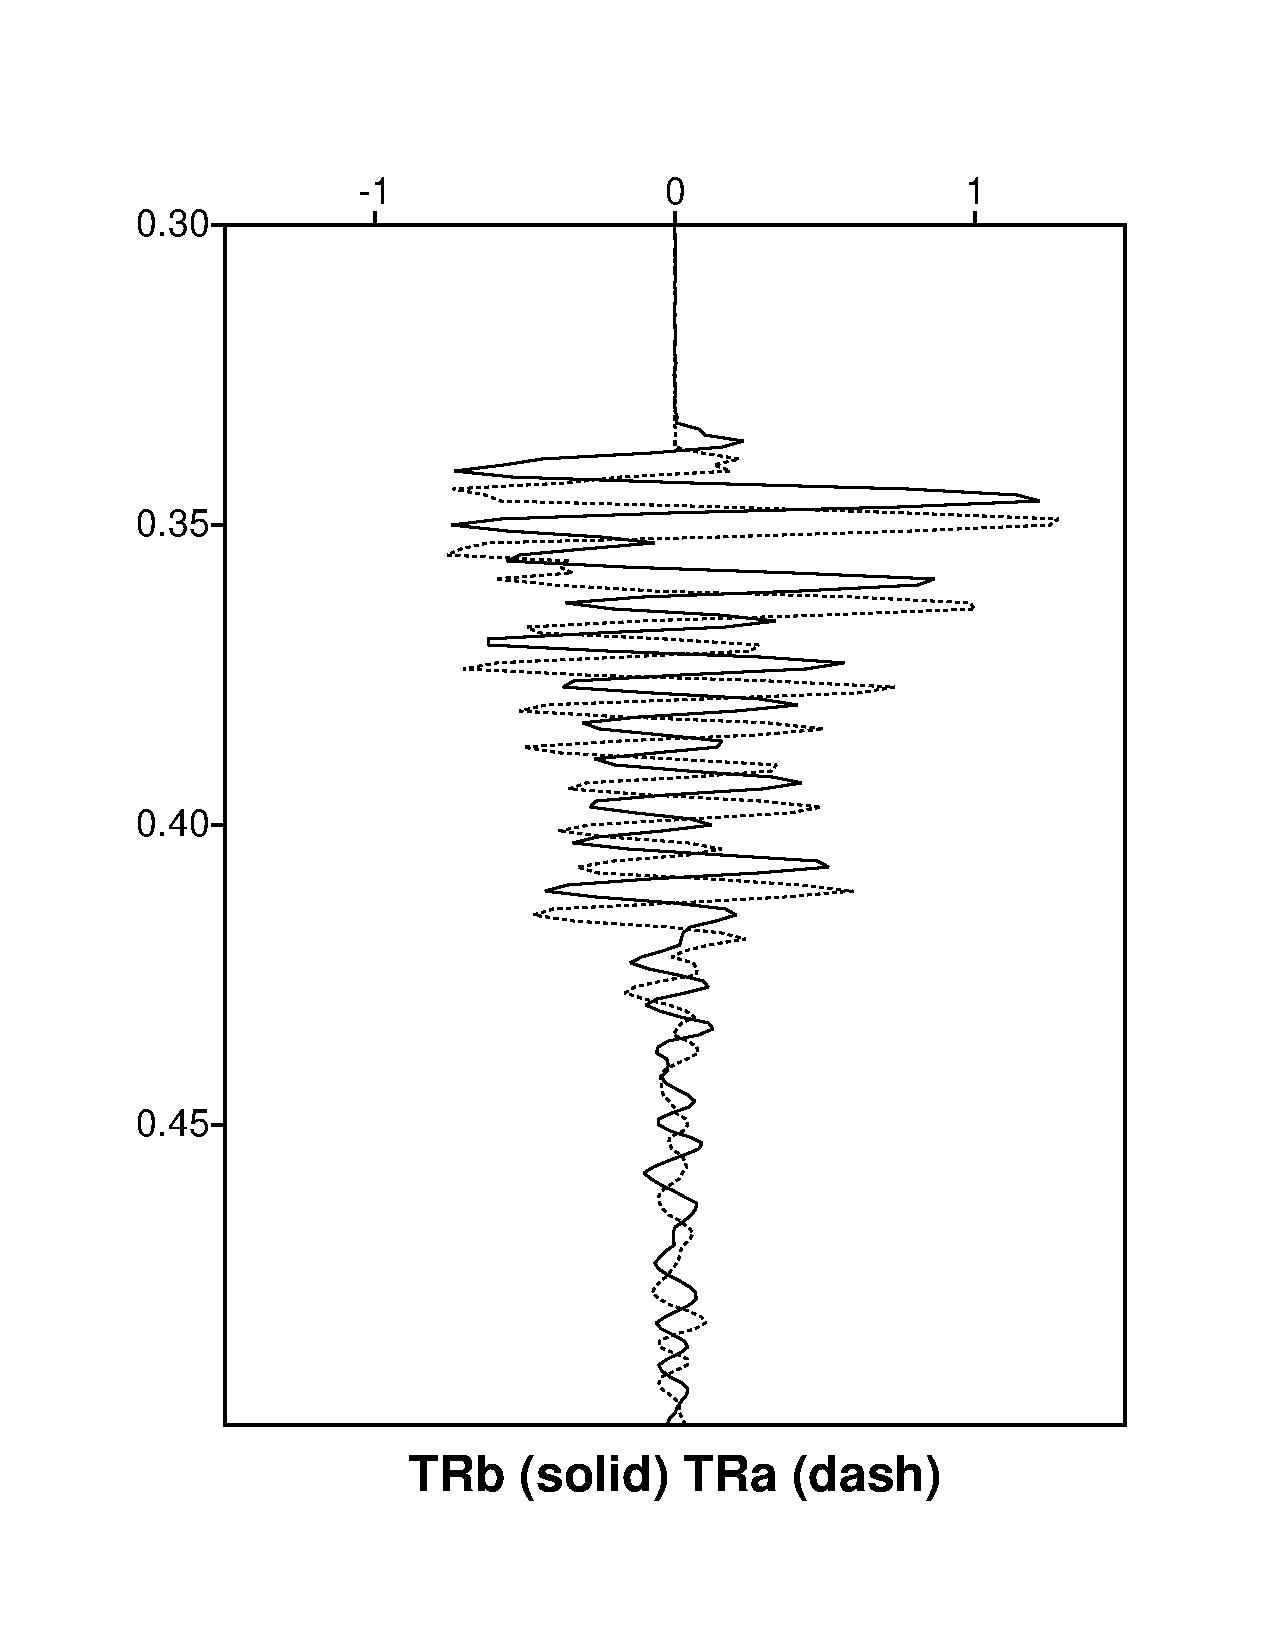
\includegraphics[width=0.45\textwidth]{Fig/fig1}
%    \label{fig:fig1}}\\
%    \subfloat[]{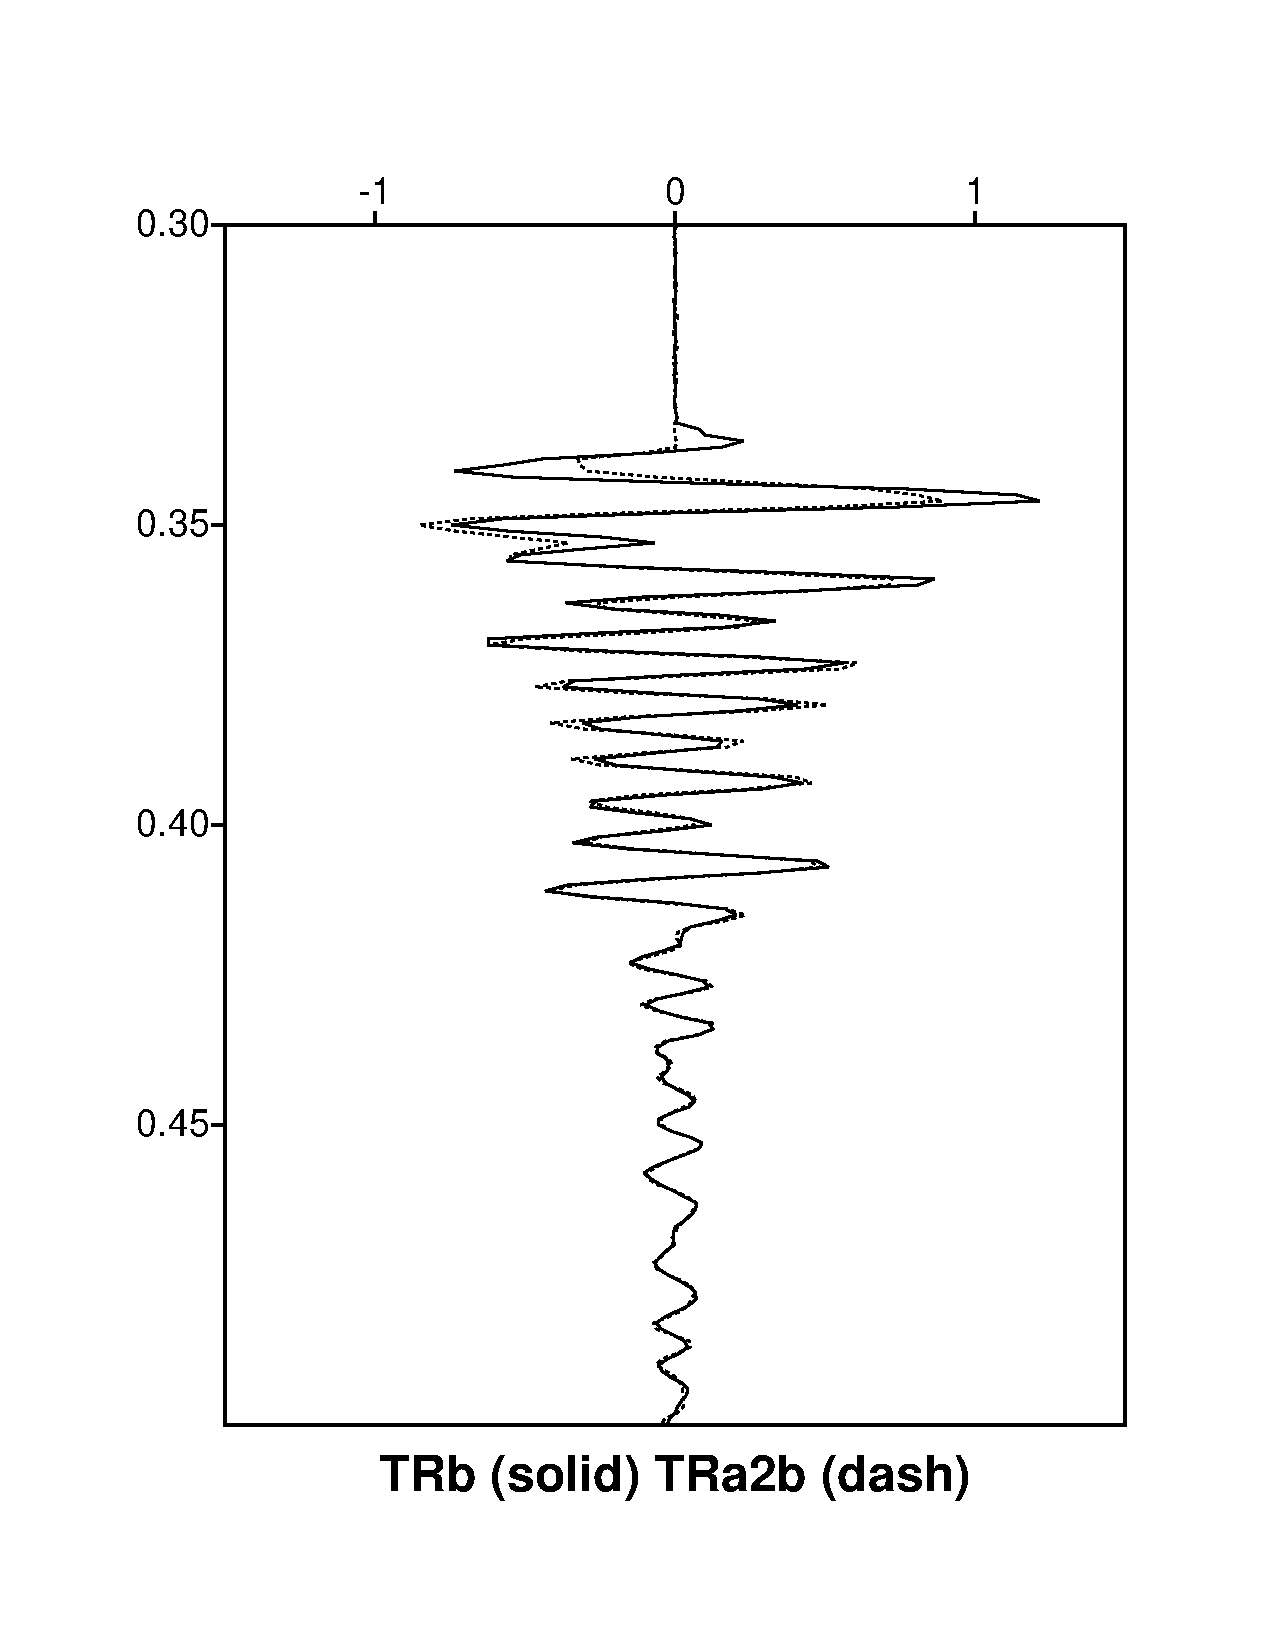
\includegraphics[width=0.45\textwidth]{Fig/fig2}
%    \label{fig:fig2}}\\
%	\caption{(a) Caption a. (b) Caption b.}
%	\label{fig:fig1,fig2}
%\end{figure}

%\begin{figure*}[ht!]
%	\centering
%	\subfloat[]{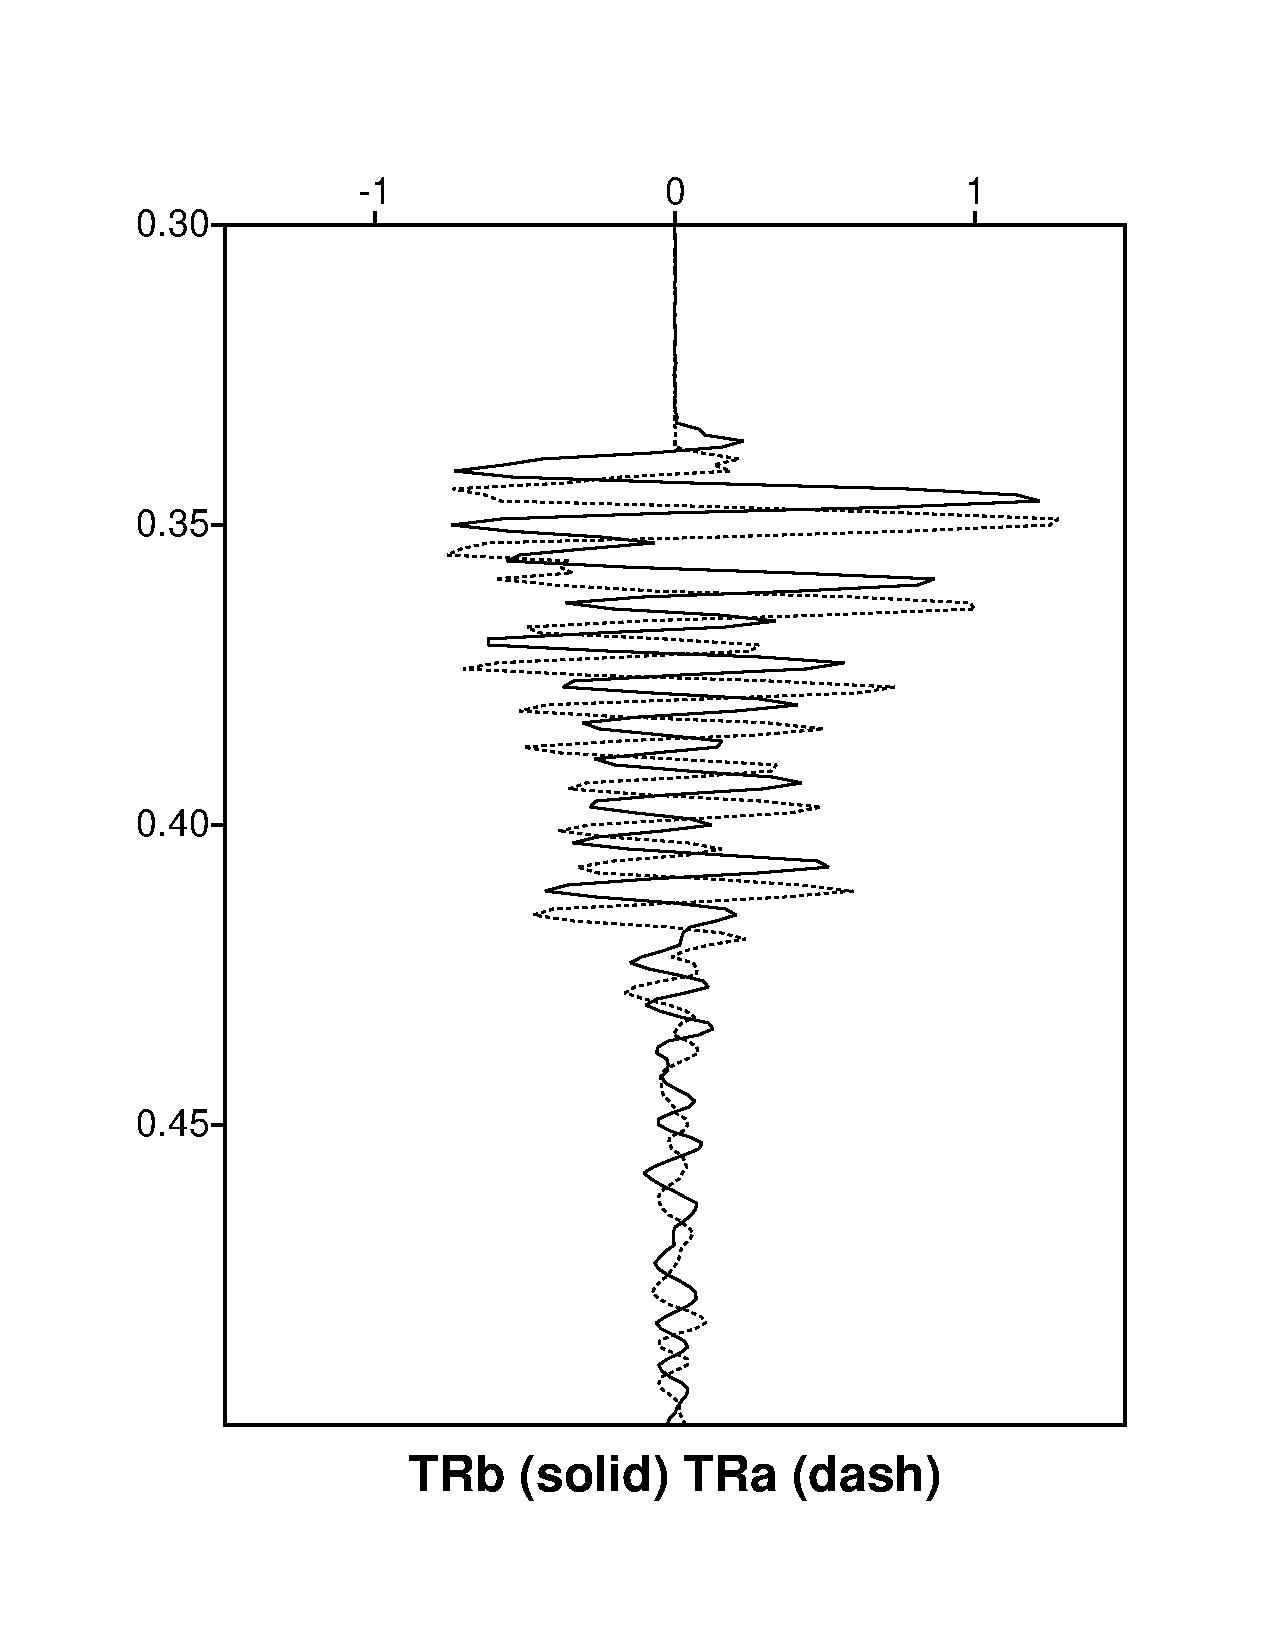
\includegraphics[width=0.45\textwidth]{Fig/fig1}
%    \label{fig:fig1}}\\
%    \subfloat[]{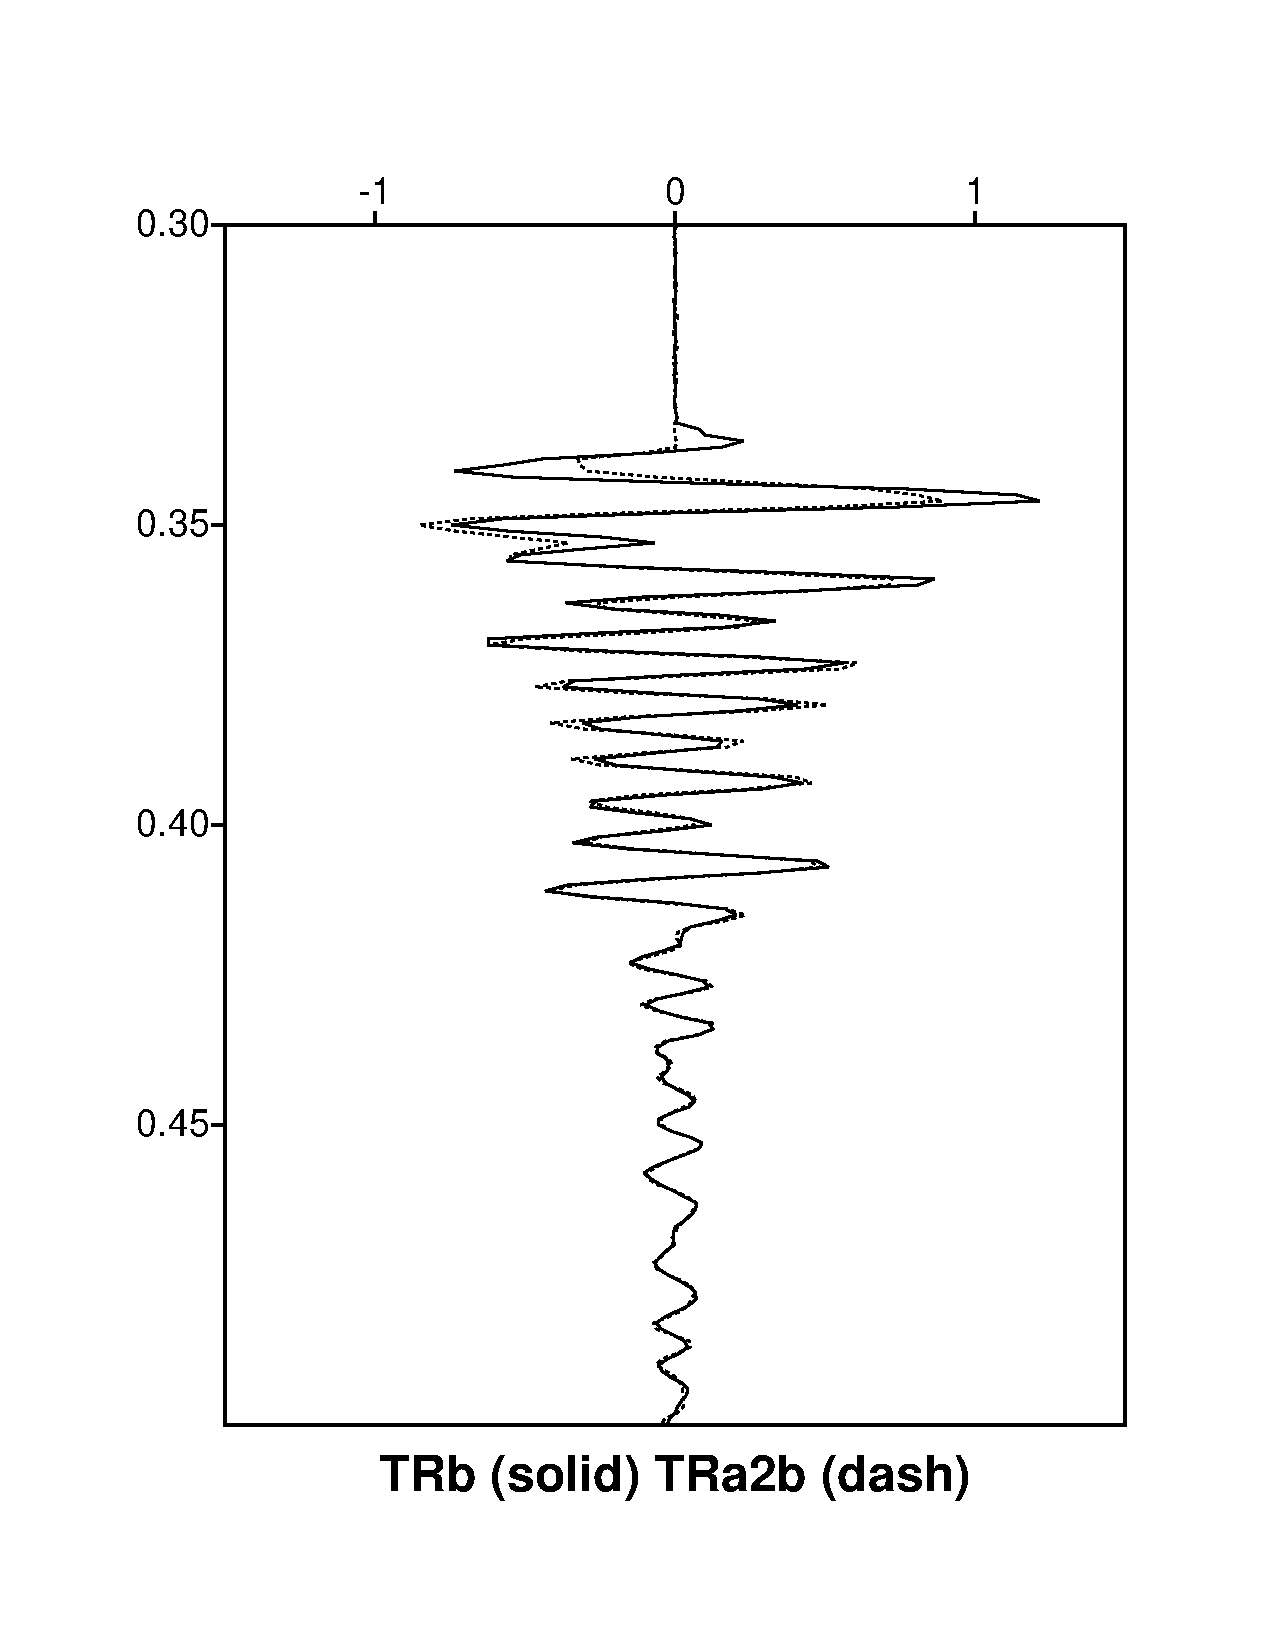
\includegraphics[width=0.45\textwidth]{Fig/fig2}
%    \label{fig:fig2}}\\
%	\caption{(a) Caption a. (b) Caption b.}
%	\label{fig:fig1,fig2}
%\end{figure*}

%\begin{table}[h]
%\caption{Table caption}
%\begin{center}
%     \begin{tabular}{|c|c|c|c|c|c|} 
%	  \hline Column1 (unit)  & Column2 (unit) & Column3 (unit) \\ 
%	  \hline 1 & 2  & 3 \\
%       \hline
%    \end{tabular} 
%\end{center}
%\label{tbl:table1}
%\end{table}

